\documentclass[letter, 10pt]{article}
\usepackage{fullpage}
\usepackage[margin=0.5in]{geometry}
\usepackage{graphicx}
\usepackage{caption}
\usepackage{subcaption}
\usepackage[table]{xcolor}
\usepackage{amsmath}
\usepackage{listings}
\usepackage{float}
\usepackage{array,multirow}
\usepackage{tikz}
\usepackage{cancel}
\usepackage{listings}
\setcounter{MaxMatrixCols}{20}
\usetikzlibrary{arrows}
\pagenumbering{gobble}
\begin{document}
\noindent
\large \textbf{Rahul Ghosh} \hfill \textbf{Assignment\#4}\\
\normalsize Student ID: 5476965 \hfill CSci 5512\\

\section*{Question 1}
\begin{itemize}
    \item[(1)] Pay of Job A lies in $\mathcal{N}(0,1)$ and the pay of job B lies in $\mathcal{N}(0.5,0.5)$. The distribution of both the pays are shown below.

    To be stochastically dominant, the area under Job A should be more than the area under Job B at all times. The total area under the curve for a normal distribution is 1. The area within 3 standard deviation is 99.6\% of the total.
    
    Even though initially the area under the curve of Job A is greater than the area under Job B, Job B has 99.6\% of its area within 2, whereas Job B has 99.6\% of its area within 3. Thus Job B does not stochastically dominate Job A. The plots of both the distribution is shown in Fig1.
    
    \begin{figure}[H]
        \centering
        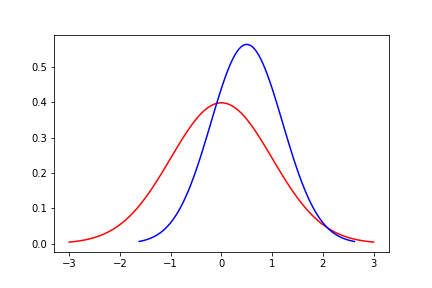
\includegraphics[width=\textwidth, height=0.4\textwidth]{HW4/P1.png}
        \caption{Distribution of Job A and Job B}
    \end{figure}
    
    \item[(2)] For Job Y to stochastically dominate Job X, $\mu_x<\mu_y$ and $\sigma^2_x<\sigma^2_y$.
    
    \item[(3)] The AUC of normal distribution is 0 at $-\infty$ and becomes 1 at $\infty$. Whereas, the AUC of uniform distribution U(a,b) becomes greater than zero at a and becomes ! at b. Therefore the normal distribution will always have more area initially and the uniform distribution will always reach area=1 before. So, neither uniform distribution stochastically dominates uniform distribution nor vice versa.
\end{itemize}

\section*{Question 2}
Since initially we don't know the machine, therefore all the machines are equally likely.
\begin{itemize}
    \item SLOT(X) $\rightarrow$ U(X) = $\frac{10}{100}\times20+\frac{30}{100}\times5+\frac{40}{100}\times1+\frac{20}{100}\times0 = 2+1.5+0.4+0 = 3.9$
    \item SLOT(Y) $\rightarrow$ U(Y) = $\frac{5}{100}\times40+\frac{25}{100}\times4+\frac{30}{100}\times2+\frac{40}{100}\times0 = 2+1+0.6+0 = 3.6$
    \item SLOT(Z) $\rightarrow$ U(Z) = $\frac{25}{100}\times10+\frac{25}{100}\times5+\frac{25}{100}\times2+\frac{25}{100}\times0 = 2.5+1.25+0.5+0 = 4.25$
\end{itemize}
$\implies U = \frac{1}{3}\times3.9+\frac{1}{3}\times3.6+\frac{1}{3}\times4.25$\\
Now, if we know the slot machines, then we will choose to play on slot machine Z since it has the highest expected utility.\\
Difference = $4.25-(\frac{1}{3}\times3.9+\frac{1}{3}\times3.6+\frac{1}{3}\times4.25) = \frac{2}{3}\times4.25 - \frac{1}{3}\times3.9+\frac{1}{3}\times3.6 = \frac{8.5-3.9-3.6}{3} = \frac{1}{3} = 0.333$\\
Therefore, we should be willing to pay 0.333\$ to get the identification done.

\section*{Question 3}
\begin{equation*}
    Reward(s) = \begin{tabular}{ |c|c|c| } 
                \hline
                \cellcolor{black}coloured & 50 & \cellcolor{black}coloured\\
                \hline
                \cellcolor{black}coloured & 0 & -3\\
                \hline
                -50 & -1 & -10\\
                \hline
                \cellcolor{black}coloured & -3 & -2\\
                \hline
                \end{tabular}\quad
    \gamma = 0.8\quad
    Probability(a) = \{0.7, 0.15, 0.15\}
\end{equation*}
\begin{itemize}
    \item[(1)] \begin{equation*}
                    Initial State = \begin{tabular}{ |c|c|c| } 
                                    \hline
                                    \cellcolor{black}coloured & 50 & \cellcolor{black}coloured\\
                                    \hline
                                    \cellcolor{black}coloured & 0 & -3\\
                                    \hline
                                    -50 & -1 & -10\\
                                    \hline
                                    \cellcolor{black}coloured & -3 & -2\\
                                    \hline
                                    \end{tabular}\quad 
                    Final State =   \begin{tabular}{ |c|c|c| } 
                                    \hline
                                    \cellcolor{black}coloured & 50 & \cellcolor{black}coloured\\
                                    \hline
                                    \cellcolor{black}coloured & 0 & -3\\
                                    \hline
                                    -50 & -1 & -10\\
                                    \hline
                                    \cellcolor{black}coloured & -3 & -2\\
                                    \hline
                                    \end{tabular}
                \end{equation*}
    \item[(2)] \begin{equation*}
                    Initial State = \begin{tabular}{ |c|c|c| } 
                                    \hline
                                    \cellcolor{black}coloured & 50 & \cellcolor{black}coloured\\
                                    \hline
                                    \cellcolor{black}coloured & 0 & 0\\
                                    \hline
                                    -50 & 0 & 0\\
                                    \hline
                                    \cellcolor{black}coloured & 0 & 0\\
                                    \hline
                                    \end{tabular}\quad 
                    Final State =   \begin{tabular}{ |c|c|c| } 
                                    \hline
                                    \cellcolor{black}coloured & 50 & \cellcolor{black}coloured\\
                                    \hline
                                    \cellcolor{black}coloured & 0 & -3\\
                                    \hline
                                    -50 & -1 & -10\\
                                    \hline
                                    \cellcolor{black}coloured & -3 & -2\\
                                    \hline
                                    \end{tabular}
                \end{equation*}
    \item[(3)]
\end{itemize}

\section*{Question 4}
\begin{equation*}
    Initial Policy = \begin{tabular}{ |c|c|c| } 
                    \hline
                    \cellcolor{black}coloured & 50 & \cellcolor{black}coloured\\
                    \hline
                    \cellcolor{black}coloured & $\uparrow$ & $\uparrow$\\
                    \hline
                    -50 & $\uparrow$ & $\uparrow$\\
                    \hline
                    \cellcolor{black}coloured & $\uparrow$ & $\uparrow$\\
                    \hline
                    \end{tabular}\quad 
    Final Policy =   \begin{tabular}{ |c|c|c| } 
                    \hline
                    \cellcolor{black}coloured & 50 & \cellcolor{black}coloured\\
                    \hline
                    \cellcolor{black}coloured & $\uparrow$ & $\leftarrow$\\
                    \hline
                    -50 & $\uparrow$ & $\uparrow$\\
                    \hline
                    \cellcolor{black}coloured & $\uparrow$ & $\uparrow$\\
                    \hline
                    \end{tabular}
\end{equation*}
\begin{equation*}
    Final Utility = \begin{tabular}{ |c|c|c| } 
                    \hline
                    \cellcolor{black}coloured & 50 & \cellcolor{black}coloured\\
                    \hline
                    \cellcolor{black}coloured & 0 & -3\\
                    \hline
                    -50 & -1 & -10\\
                    \hline
                    \cellcolor{black}coloured & -3 & -2\\
                    \hline
                    \end{tabular}
\end{equation*}

\section*{Question 5}
Let,
$b(s) = \begin{tabular}{ |c|c| } 
                    \hline
                    a & b\\
                    \hline
                    c & d\\
                    \hline
                \end{tabular},\quad
Probability(a) = \{0.7, 0.15, 0.15\}\quad
P(e|s) = \begin{tabular}{ |c|c| } 
            \hline
            0.3 & 0\\
            \hline
            0.9 & 0.2\\
            \hline
        \end{tabular}\quad
b(s') = \begin{tabular}{ |c|c| } 
            \hline
            A & B\\
            \hline
            C & D\\
            \hline
        \end{tabular}$
\\

Suppose the chosen action is "LEFT". Then,\\
$
A = 0.3\times (0.85\times a + 0.7\times b + 0.15\times c + 0\times d)\\
B = 0\times (0\times a + 0.15\times b + 0\times c + 0.15\times d)\\
C = 0.9\times (0.15\times a + 0\times b + 0.85\times c + 0.7\times d)\\
D = 0.2\times (0\times a + 0.15\times b + 0\times c + 0.15\times d)\\
$

Similarly if the chosen action is "RIGHT". Then,\\
$
A = 0.3\times (0.15\times a + 0.15\times b + 0\times c + 0\times d)\\
B = 0\times (0.15\times a + 0.15\times b + 0\times c + 0\times d)\\
C = 0.9\times (0.7\times a + 0\times b + 0.85\times c + 0.15\times d)\\
D = 0.2\times(0\times a + 0.7\times b + 0.15\times c + 0.85\times d)
$
\\

The sequence of actions for this problem can be
\begin{itemize}
    \item[1] LEFT, DOWN
    $\implies   \begin{tabular}{ |c|c| } 
                    \hline
                    0.2 & 0.3\\
                    \hline
                    0 & 0.5\\
                    \hline
                \end{tabular} \xrightarrow{\text{LEFT}}
                \begin{tabular}{ |c|c| } 
                    \hline
                    0.114 & 0\\
                    \hline
                    0.342 & 0.0024\\
                    \hline
                \end{tabular} \xrightarrow{\text{DOWN}}
                \begin{tabular}{ |c|c| } 
                    \hline
                    0.00513 & 0\\
                    \hline
                    0.33669 & 0.01434\\
                    \hline
                \end{tabular}\implies$
    REWARD = 0.30288
    \item[2] LEFT, LEFT
    $\implies   \begin{tabular}{ |c|c| } 
                    \hline
                    0.2 & 0.3\\
                    \hline
                    0 & 0.5\\
                    \hline
                \end{tabular} \xrightarrow{\text{LEFT}}
                \begin{tabular}{ |c|c| } 
                    \hline
                    0.114 & 0\\
                    \hline
                    0.342 & 0.0024\\
                    \hline
                \end{tabular} \xrightarrow{\text{LEFT}}
                \begin{tabular}{ |c|c| } 
                    \hline
                    0.04446 & 0\\
                    \hline
                    0.29214 & 0.00072\\
                    \hline
                \end{tabular}\implies$
    REWARD = 0.24624
    \item[3] DOWN, LEFT
    $\implies   \begin{tabular}{ |c|c| } 
                    \hline
                    0.2 & 0.3\\
                    \hline
                    0 & 0.5\\
                    \hline
                \end{tabular} \xrightarrow{\text{DOWN}}
                \begin{tabular}{ |c|c| } 
                    \hline
                    0.0225 & 0\\
                    \hline
                    0.1935 & 0.127\\
                    \hline
                \end{tabular} \xrightarrow{\text{LEFT}}
                \begin{tabular}{ |c|c| } 
                    \hline
                    0.014445 & 0\\
                    \hline
                    0.231075 & 0.00381\\
                    \hline
                \end{tabular}\implies$
    REWARD = 0.20901
    \item[4] DOWN, DOWN
    $\implies   \begin{tabular}{ |c|c| } 
                    \hline
                    0.2 & 0.3\\
                    \hline
                    0 & 0.5\\
                    \hline
                \end{tabular} \xrightarrow{\text{DOWN}}
                \begin{tabular}{ |c|c| } 
                    \hline
                    0.0225 & 0\\
                    \hline
                    0.1935 & 0.127\\
                    \hline
                \end{tabular} \xrightarrow{\text{DOWN}}
                \begin{tabular}{ |c|c| } 
                    \hline
                    0.00101 & 0\\
                    \hline
                    0.17935 & 0.0274\\
                    \hline
                \end{tabular}\implies$
    REWARD = 0.123545
\end{itemize}
Thus, \{LEFT, DOWN\} is the best sequence of actions that can be taken.
\end{document}